\chapter{Assessment}\label{chp:assessment}

\section{Introduction}

This chapter will discuss the implementatons in the previous chapter. Intended functionality and performance is compared to the actual results, and usefullness in the context of autonomous navigation is assessed. The assesments will be mostly qualitative in nature.

\section{Vanishing Point Detection}

The vanishing point detector failed work as intended. Both the \gls{dsam} algorithm and the vanishing point detector itself is unable to fulfill their intended tasks. 

\section{What Does Work?}

The application is stable and responsive as long as the \gls{dsam} algorithm is left out. While eliminating all errors and bugs was too time consuming to be completed, testing showed that the vanishing point voting scheme is working properly. It is suspected that the error is caused by mixing two coordinate systems.

\section{Depth Perception and Obstruction Detection}

\subsection{Stereo Vision}

The stereo matching process has two significant weaknesses: inability to detect textureless surfaces, and false disparities from repetitive patterns. It may be that the matching parameters can be tuned in order to achieve denser disparity maps. On the other hand, the input images from the IP cameras are quite noisy, which makes the matching process much more difficult. It is possible that areas of the images where the distictive features are faint are especially sensitive to noise. This results in a sparse disparity map, which can be unsuitable in applications such as 3d reconstruction and mapping of the environment.

\begin{figure}
	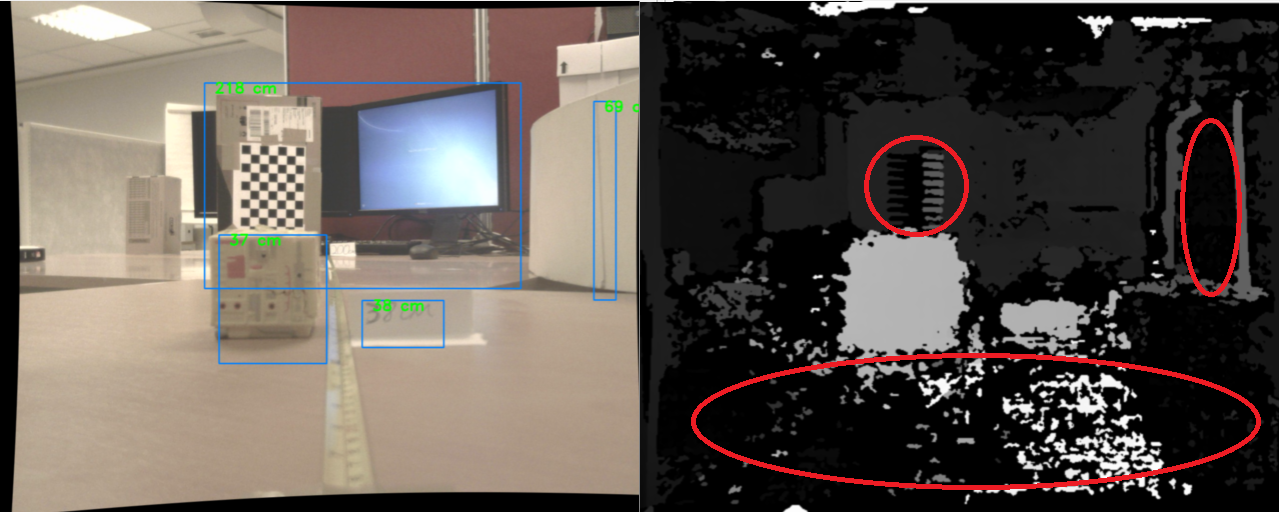
\includegraphics[width=\textwidth]{stereoWeakness}
	\caption{Illustration of the weaknesses with stereo matching. Little or no matching where there are few distict features. False matches and shadows caused by reperitive patterns.}
	\label{fig:stereoWeakness}
\end{figure}

\subsection{Obstacle Detection}



Obstacle detection based on depth layers works as intended, and could potentially be adapted and improved for an obstacle avoidance system. Figure \ref{fig:contourDetection} in chapter \ref{chp:implementation} shows that several contours are placed closed to each other, thus resulting in an image cluttered with detected obstructions. While a cluttered image is not user friendly, it is not necessarily a problem in terms of obstacle detection. Note that this is an obstacle detector, not an object detector. This implies that it is sufficient to know that something is obstructing the path of the robot. 


